% ML APIs and Software Stack
% Standalone section fragment for the existing Machine Learning Foundations textbook.
% Assumes the book preamble already provides: amsmath, booktabs, tabularx, array, tikz,
% and the existing callout environments used elsewhere in the textbook.

\chapter{ML APIs and the Software Stack}
\label{sec:ml-apis}

The useful question is not ``which ML library should I memorise?'' but \textbf{which layer of the system is this software responsible for?}
PyTorch, CUDA, vLLM, MLflow, Ray, Bedrock and LangGraph solve different problems and often appear in the same pipeline.
Treating them as competitors hides the architecture.

A compact mental model is
\[
\boxed{
\text{application}
\rightarrow
\text{model/runtime}
\rightarrow
\text{compiler/kernels}
\rightarrow
\text{hardware}
}
\]
with distributed execution, experiment state and deployment infrastructure cutting across those layers.

\begin{figure}[ht]
\centering
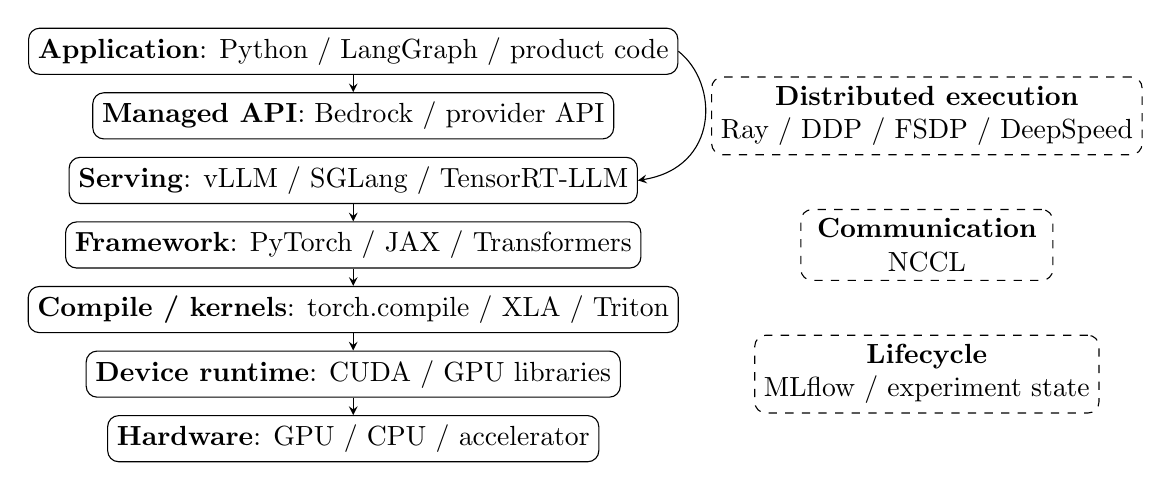
\begin{tikzpicture}[x=1.55cm,y=0.82cm,>=stealth]
\node[draw,rounded corners,minimum width=4.1cm,minimum height=0.55cm] (app) at (0,5.8)
{\textbf{Application}: Python / LangGraph / product code};
\node[draw,rounded corners,minimum width=4.1cm,minimum height=0.55cm] (api) at (0,4.8)
{\textbf{Managed API}: Bedrock / provider API};
\node[draw,rounded corners,minimum width=4.1cm,minimum height=0.55cm] (serve) at (0,3.8)
{\textbf{Serving}: vLLM / SGLang / TensorRT-LLM};
\node[draw,rounded corners,minimum width=4.1cm,minimum height=0.55cm] (framework) at (0,2.8)
{\textbf{Framework}: PyTorch / JAX / Transformers};
\node[draw,rounded corners,minimum width=4.1cm,minimum height=0.55cm] (compile) at (0,1.8)
{\textbf{Compile / kernels}: torch.compile / XLA / Triton};
\node[draw,rounded corners,minimum width=4.1cm,minimum height=0.55cm] (cuda) at (0,0.8)
{\textbf{Device runtime}: CUDA / GPU libraries};
\node[draw,rounded corners,minimum width=4.1cm,minimum height=0.55cm] (gpu) at (0,-0.2)
{\textbf{Hardware}: GPU / CPU / accelerator};

\draw[->] (app) -- (api);
\draw[->] (app.east) .. controls (3.0,5.3) and (3.0,4.0) .. (serve.east);
\draw[->] (serve) -- (framework);
\draw[->] (framework) -- (compile);
\draw[->] (compile) -- (cuda);
\draw[->] (cuda) -- (gpu);

\node[draw,dashed,rounded corners,align=center,minimum width=3.2cm] at (4.7,4.8)
{\textbf{Distributed execution}\\Ray / DDP / FSDP / DeepSpeed};
\node[draw,dashed,rounded corners,align=center,minimum width=3.2cm] at (4.7,2.8)
{\textbf{Communication}\\NCCL};
\node[draw,dashed,rounded corners,align=center,minimum width=3.2cm] at (4.7,0.8)
{\textbf{Lifecycle}\\MLflow / experiment state};
\end{tikzpicture}
\caption{The ML software stack is a set of abstraction boundaries.
Most tools occupy one layer while orchestration, communication and lifecycle systems cut across several layers.}
\label{fig:ml-api-stack}
\end{figure}

\begin{calloutmemoryhook}
Every ML API chooses an abstraction boundary: decide what you want to control and what you want somebody else to solve.
\end{calloutmemoryhook}

\subsection{Start with the problem, not the product}

The same model can move through several APIs because each one removes a different kind of work.
A useful first classification is therefore by \textbf{problem solved}.

\begin{table}[ht]
\centering
\small
\begin{tabularx}{\textwidth}{>{\bfseries}p{2.6cm} X X}
\toprule
Problem & Natural tools & What the abstraction makes easier \\
\midrule
Numerical algorithms & NumPy, SciPy & arrays, linear algebra, optimisation, integration, statistics \\
Model programming & PyTorch, JAX & autodiff, parameterised models, accelerator execution \\
Pretrained models & Transformers & loading model architectures, tokenisers and checkpoints behind common interfaces \\
Compilation & \texttt{torch.compile}, XLA & fuse and lower larger computation graphs rather than dispatching every operation independently \\
GPU kernels & Triton, CUDA & control how an operation maps to accelerator hardware \\
GPU communication & NCCL & collective tensor communication between GPUs \\
Distributed training & DDP, FSDP, DeepSpeed, Ray Train & replicate, shard and schedule training work \\
LLM inference & vLLM, SGLang, TensorRT-LLM & KV-cache management, request scheduling and efficient decoding \\
Model serving & Triton Inference Server, Ray Serve, KServe-like systems & expose one or more models as network services \\
Experiment lifecycle & MLflow, W\&B-like systems & runs, metrics, artifacts, lineage and model versions \\
Managed foundation models & Bedrock-like APIs & consume models without operating the inference stack \\
Agent workflows & LangGraph-like systems & explicit state, branching, retries and tool-calling workflows \\
\bottomrule
\end{tabularx}
\caption{Different tools are usually answers to different systems problems rather than substitutes for one another.}
\label{tab:ml-api-problems}
\end{table}

The \textbf{inductive bias} of an API is the workflow it assumes should be cheap.
PyTorch assumes model computation can be expressed as tensor operations plus automatic differentiation.
vLLM assumes many autoregressive requests should share expensive accelerator memory efficiently.
MLflow assumes experiment identity and lineage must survive beyond the Python process that produced them.
Bedrock assumes the user values a stable managed model interface more than direct ownership of the serving stack.

\begin{calloutinductivebias}
If the abstraction matches the dominant operation, it removes low-value engineering work; if the abstraction hides a variable you need to control, it becomes a restriction.
\end{calloutinductivebias}


\subsection{Numerical computing: NumPy and SciPy}

\textbf{NumPy} gives Python a typed multidimensional-array model.
The useful systems idea is that a numerical object is not a Python list of independent values but an array with shape, dtype, strides and contiguous memory behaviour, matching the tensor discussion in Section~2.3.1.

\textbf{SciPy} builds higher-level numerical algorithms around NumPy-compatible arrays.
Its role is not specifically ``machine learning''; it provides established implementations of operations such as optimisation, root finding, numerical integration, sparse linear algebra, interpolation, signal processing and statistics.

The data flow is usually
\[
\underbrace{\text{array-valued problem}}_{\text{NumPy representation}}
\rightarrow
\underbrace{\text{specialised numerical routine}}_{\text{SciPy}}
\rightarrow
\underbrace{\text{solution / statistic / transformed array}}_{\text{returned to Python}}.
\]

For example, a scientific ML project may use PyTorch for a learned surrogate while using \texttt{scipy.optimize} to fit a small classical calibration problem or \texttt{scipy.integrate} to evaluate a reference calculation.
The boundary is therefore \textbf{general numerical algorithm} versus \textbf{learned differentiable model} rather than old versus modern.

\begin{table}[ht]
\centering
\small
\begin{tabularx}{\textwidth}{>{\bfseries}p{2.3cm} X X X}
\toprule
Tool & Natural unit & Strength & Main cost / limitation \\
\midrule
NumPy & array & simple CPU numerical programming and interoperability & no general neural-network training/runtime layer \\
SciPy & numerical problem + arrays & mature specialised algorithms & usually not the accelerator/autodiff layer for large neural models \\
PyTorch / JAX & tensors / transformed numerical functions & autodiff and accelerator-oriented ML computation & heavier runtime and different execution semantics \\
\bottomrule
\end{tabularx}
\caption{NumPy/SciPy and ML frameworks overlap numerically but optimise for different workflows.}
\end{table}


\subsection{Model programming: PyTorch and JAX}

\subsubsection*{PyTorch: tensors, autograd and modules}

PyTorch normally receives tensors, executes tensor operations, records the differentiable computation required by autograd, and produces gradients used by an optimiser:
\[
\underbrace{X}_{\text{input tensors}}
\rightarrow
\underbrace{f_{\theta_{\text{weights}}}(X)}_{\text{tensor operations}}
\rightarrow
\underbrace{\mathcal{L}}_{\text{scalar objective}}
\rightarrow
\underbrace{\frac{\partial \mathcal{L}}{\partial \theta_{\text{weights}}}}_{\text{autograd}}
\rightarrow
\underbrace{\theta_{\text{weights}}\leftarrow\text{optimiser update}}_{\text{Section 7}}.
\]

The abstraction is attractive because the forward model can be written in ordinary Python while tensor/device semantics remain explicit enough for research.
The cost is that Python flexibility can obstruct whole-program optimisation: a compiler can only optimise the computation it can successfully capture.

\texttt{torch.compile} changes that boundary.
Instead of dispatching each PyTorch operation independently, it attempts to capture compilable regions and lower them through a backend such as TorchInductor into optimised kernels.
Graph breaks return execution to ordinary Python, preserving flexibility but losing some optimisation opportunity.

\begin{figure}[ht]
\centering
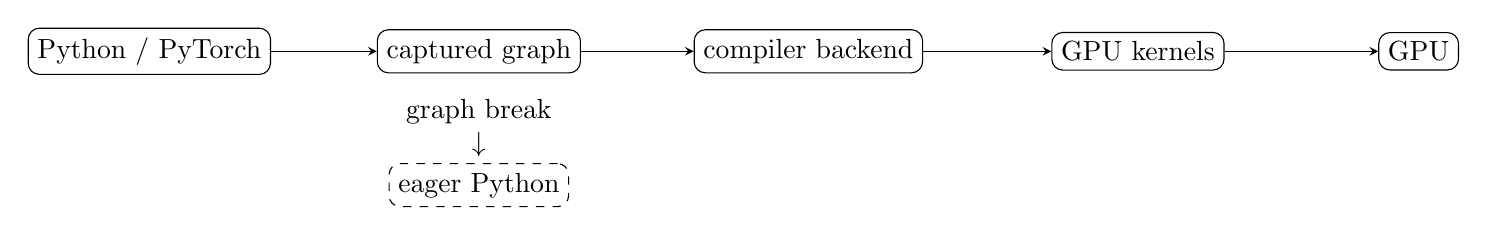
\begin{tikzpicture}[x=1.55cm,y=0.85cm,>=stealth]
\node[draw,rounded corners] (py) at (0,2) {Python / PyTorch};
\node[draw,rounded corners] (graph) at (2.7,2) {captured graph};
\node[draw,rounded corners] (inductor) at (5.4,2) {compiler backend};
\node[draw,rounded corners] (kernel) at (8.1,2) {GPU kernels};
\node[draw,rounded corners] (gpu) at (10.4,2) {GPU};

\draw[->] (py) -- (graph);
\draw[->] (graph) -- (inductor);
\draw[->] (inductor) -- (kernel);
\draw[->] (kernel) -- (gpu);

\node[align=center] at (2.7,0.85) {graph break\\$\downarrow$};
\node[draw,dashed,rounded corners] at (2.7,0) {eager Python};
\end{tikzpicture}
\caption{\texttt{torch.compile} moves part of the execution path from operation-by-operation dispatch toward graph-level compilation while retaining an eager fallback.}
\label{fig:torch-compile}
\end{figure}

\begin{calloutpracticaltip}
Profile before writing custom kernels: first remove Python/graph overhead with the framework compiler, then replace an operation only if the kernel itself remains the bottleneck.
\end{calloutpracticaltip}

\subsubsection*{JAX: functions plus transformations}

JAX starts from a different programming model.
A numerical function is written using JAX operations and then transformed:

\[
\underbrace{f}_{\text{numerical function}}
\overset{\texttt{grad}}{\longrightarrow}
\underbrace{\nabla f}_{\text{differentiate}},
\qquad
\underbrace{f}_{\text{one-example function}}
\overset{\texttt{vmap}}{\longrightarrow}
\underbrace{f_{\text{batched}}}_{\text{vectorise}},
\qquad
\underbrace{f}_{\text{Python/JAX function}}
\overset{\texttt{jit}}{\longrightarrow}
\underbrace{f_{\text{compiled}}}_{\text{lower to accelerator executable}}.
\]

The transformations compose, which encourages functions whose outputs depend explicitly on their inputs rather than hidden mutable state.
That restriction gives compilers more freedom to trace, fuse, vectorise and place operations.

\begin{table}[ht]
\centering
\small
\begin{tabularx}{\textwidth}{>{\bfseries}p{2.1cm} X X}
\toprule
 & PyTorch & JAX \\
\midrule
Primary mental model & tensor program + modules + dynamic autograd & numerical functions + composable transformations \\
Differentiation & autograd over tensor operations & \texttt{grad} transforms functions \\
Compilation & optional \texttt{torch.compile} capture around flexible Python & \texttt{jit} is a first-class function transformation \\
Batching & usually explicit batch dimensions / framework operators & \texttt{vmap} can transform single-example code into batched code \\
State style & object/module state is natural & explicit functional state is strongly favoured \\
Strength & flexible research/debugging ecosystem & transformation/composition and accelerator-oriented functional programming \\
Cost & Python dynamism can block compilation & transformed code has stricter tracing/purity constraints \\
\bottomrule
\end{tabularx}
\caption{PyTorch and JAX overlap strongly in capability but expose different programming biases.}
\label{tab:pytorch-jax}
\end{table}

\begin{calloutmemoryhook}
PyTorch starts from tensor programs and adds compilation; JAX starts from transformable numerical functions.
\end{calloutmemoryhook}


\subsection{Pretrained-model APIs: Transformers and Accelerate}

The Hugging Face \textbf{Transformers} ecosystem mainly removes repeated model-specific interface work.
Instead of writing a different loading and tokenisation path for every architecture, a user can often express

\[
\text{model identifier}
\rightarrow
\text{configuration + tokenizer + weights}
\rightarrow
\text{framework model}
\rightarrow
\text{training or inference}.
\]

The library therefore sits \emph{above} PyTorch/JAX rather than replacing them.
The checkpoint and architecture interface becomes standardised while the actual tensor computation still runs through the underlying framework.

\textbf{Accelerate} removes a different class of repetition: device placement and distributed-training setup.
It can configure a training loop around backends such as DDP, FSDP or DeepSpeed while keeping much of the user training code unchanged.

\begin{figure}[ht]
\centering
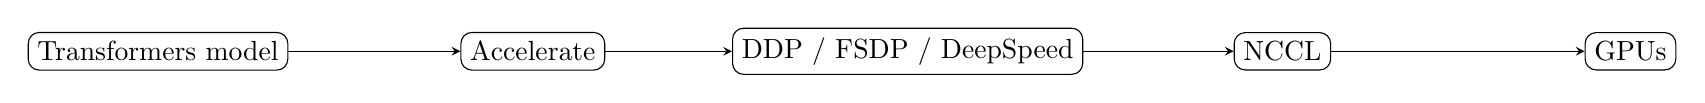
\begin{tikzpicture}[x=1.7cm,y=0.85cm,>=stealth]
\node[draw,rounded corners] (model) at (0,2.5) {Transformers model};
\node[draw,rounded corners] (accel) at (2.8,2.5) {Accelerate};
\node[draw,rounded corners] (backend) at (5.6,2.5) {DDP / FSDP / DeepSpeed};
\node[draw,rounded corners] (comm) at (8.4,2.5) {NCCL};
\node[draw,rounded corners] (gpus) at (11.0,2.5) {GPUs};

\draw[->] (model) -- (accel);
\draw[->] (accel) -- (backend);
\draw[->] (backend) -- (comm);
\draw[->] (comm) -- (gpus);
\end{tikzpicture}
\caption{A convenience API can sit above a distributed backend, which itself sits above the communication runtime.}
\label{fig:accelerate-stack}
\end{figure}

This distinction generalises: \textbf{high-level training libraries configure lower-level runtimes; they do not make those runtimes disappear.}


\subsection{From Python to GPU: compiler, kernel and runtime}

A GPU calculation crosses several abstraction layers:

\[
\text{Python model}
\rightarrow
\text{framework graph}
\rightarrow
\text{compiler}
\rightarrow
\text{kernel}
\rightarrow
\text{CUDA runtime / libraries}
\rightarrow
\text{GPU}.
\]

The layers matter because ``the model is slow'' can mean different things:
too many Python dispatches, poor graph fusion, an inefficient kernel, excessive memory traffic, low occupancy, or communication between devices.

\subsubsection*{CUDA}

CUDA is NVIDIA's GPU programming platform and programming model.
At the useful conceptual level, host code allocates/transfers data, launches kernels, and coordinates work executed by many GPU threads.

The low-level advantage is \textbf{control}.
The programmer can reason directly about thread/block decomposition, memory hierarchy, synchronisation and device-specific behaviour.
The cost is that performance portability and correctness become the programmer's problem.

\subsubsection*{Triton language}

Triton is a Python-based language/compiler for writing custom parallel GPU kernels.
It exposes block-wise tensor operations at a higher level than CUDA C++ while still allowing the programmer to choose how data is tiled and loaded.

A matrix operation can therefore be expressed at three useful levels:

\begin{table}[ht]
\centering
\small
\begin{tabularx}{\textwidth}{>{\bfseries}p{2.4cm} X X X}
\toprule
Level & What the programmer expresses & Main benefit & Main cost \\
\midrule
PyTorch/JAX op & desired tensor operation & fastest development and portability & least direct control over generated kernel \\
Triton kernel & block/tile-level data movement and computation & custom kernels without full CUDA complexity & kernel tuning still required \\
CUDA C++ & threads, blocks, memory and synchronisation close to hardware & maximum direct control & highest implementation/debugging cost \\
\bottomrule
\end{tabularx}
\caption{Kernel APIs trade implementation effort against control rather than forming a universal speed ranking.}
\label{tab:kernel-layers}
\end{table}

Triton is not automatically faster than a framework kernel, and CUDA is not automatically faster than Triton.
A mature vendor/library kernel may already be close to the hardware limit.
The relevant question is whether the current abstraction prevents an optimisation the workload needs.

\begin{calloutintuition}
Move down the stack only when the higher layer hides a performance decision that matters.
\end{calloutintuition}

\subsubsection*{Compiler evolution}

The recurring pressure has been to retain high-level model code while recovering low-level performance:

\begin{table}[ht]
\centering
\small
\begin{tabularx}{\textwidth}{>{\bfseries}p{2.3cm} X X X}
\toprule
Step & What changed & Problem targeted & New trade-off \\
\midrule
Eager framework & execute operations as Python asks for them & flexible research iteration & repeated dispatch + limited cross-op optimisation \\
Graph/JIT compilation & capture larger regions before execution & fusion, dispatch overhead, global optimisation & tracing restrictions and compile time \\
Generated/custom kernels & specialise important operations & memory traffic / operation-specific inefficiency & tuning and hardware dependence \\
Low-level GPU code & expose execution details directly & remaining kernel-level bottlenecks & development and maintenance complexity \\
\bottomrule
\end{tabularx}
\caption{Compilation pushes the abstraction boundary downward only where performance justifies the added constraints.}
\end{table}


\subsection{GPU communication: NCCL}

Once one logical model spans multiple GPUs, computation is no longer the only cost.
Workers must exchange parameters, gradients, activations or expert traffic.

\textbf{NCCL} provides GPU-oriented collective communication operations.
For example, an AllReduce with sum semantics maps local arrays
\[
g^{(1)},g^{(2)},\ldots,g^{(N_{\text{GPUs}})}
\]
to the same aggregate on every participating rank:
\[
\underbrace{g^{(k)}_{\text{after}}}_{\text{available on every GPU}}
=
\underbrace{\sum_{j=1}^{N_{\text{GPUs}}} g^{(j)}_{\text{before}}}_{\text{combined contribution from all GPUs}}.
\]

This is the communication pattern behind ordinary data-parallel gradient synchronisation.
Other collectives include broadcast, AllGather and ReduceScatter.

\begin{figure}[ht]
\centering
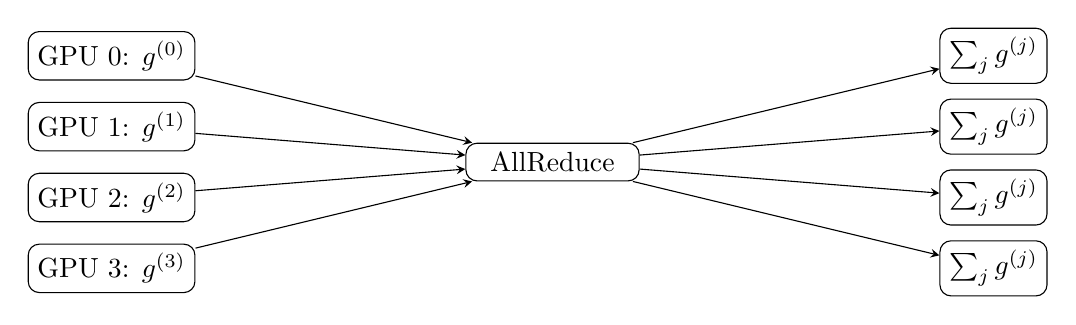
\begin{tikzpicture}[x=1.4cm,y=0.9cm,>=stealth]
\node[draw,rounded corners] (g0) at (0,3) {GPU 0: $g^{(0)}$};
\node[draw,rounded corners] (g1) at (0,2) {GPU 1: $g^{(1)}$};
\node[draw,rounded corners] (g2) at (0,1) {GPU 2: $g^{(2)}$};
\node[draw,rounded corners] (g3) at (0,0) {GPU 3: $g^{(3)}$};

\node[draw,rounded corners,minimum width=2.2cm] (ar) at (4.0,1.5) {AllReduce};

\node[draw,rounded corners] (o0) at (8,3) {$\sum_j g^{(j)}$};
\node[draw,rounded corners] (o1) at (8,2) {$\sum_j g^{(j)}$};
\node[draw,rounded corners] (o2) at (8,1) {$\sum_j g^{(j)}$};
\node[draw,rounded corners] (o3) at (8,0) {$\sum_j g^{(j)}$};

\draw[->] (g0) -- (ar);
\draw[->] (g1) -- (ar);
\draw[->] (g2) -- (ar);
\draw[->] (g3) -- (ar);
\draw[->] (ar) -- (o0);
\draw[->] (ar) -- (o1);
\draw[->] (ar) -- (o2);
\draw[->] (ar) -- (o3);
\end{tikzpicture}
\caption{AllReduce combines values across ranks and returns the aggregate to every rank.}
\label{fig:nccl-allreduce}
\end{figure}

NCCL does not decide the training algorithm.
DDP/FSDP/DeepSpeed decide \emph{which tensors need communication and when}; NCCL performs many of the GPU-to-GPU collective operations efficiently.

\begin{calloutmemoryhook}
Distributed framework decides what must move; NCCL moves it.
\end{calloutmemoryhook}


\subsection{Distributed training: DDP, FSDP, DeepSpeed and Ray}

These tools are often grouped together despite controlling different parts of the system.

\subsubsection*{DDP: replicate model, split data}

Distributed Data Parallel keeps a model replica on each worker.
Each worker processes different data, computes local gradients, and synchronises them before the optimiser update.

\[
\underbrace{B_{\text{global}}}_{\text{examples per optimisation step}}
=
\underbrace{B_{\text{device}}}_{\text{examples per worker}}
\times
\underbrace{N_{\text{workers}}}_{\text{model replicas}}.
\]

The attraction is simplicity and high throughput when the complete model plus optimiser state fits on each GPU.
The limitation is duplicated model state.

\subsubsection*{FSDP: shard model state}

Fully Sharded Data Parallel reduces replication by distributing parameters, gradients and optimiser state across workers, materialising what is required for computation at the appropriate point.

The useful trade is
\[
\boxed{
\text{less per-GPU model state}
\leftrightarrow
\text{more communication + orchestration}
}.
\]

This allows larger models to fit but makes communication schedule, sharding policy and overlap with compute important.

\subsubsection*{DeepSpeed}

DeepSpeed provides a wider runtime around large-model training, including ZeRO-style state partitioning, offload options and other large-scale training optimisations.
Its useful distinction from FSDP is not simply ``better sharding''; it is a broader training system with its own configuration/runtime choices.

\subsubsection*{Ray}

Ray operates at a different level.
Its core primitives are \textbf{tasks}, which execute functions asynchronously, and \textbf{actors}, which are stateful workers.
Resource requirements such as CPUs and GPUs become scheduler inputs.

This means Ray can coordinate work that is larger than one training collective:
hyperparameter trials, data-processing jobs, distributed training workers, model-serving replicas, or heterogeneous application tasks.

\begin{table}[ht]
\centering
\small
\begin{tabularx}{\textwidth}{>{\bfseries}p{2.0cm} X X X}
\toprule
System & Primary decision & Best mental model & Main new cost \\
\midrule
DDP & which data each replica processes & replicate model, synchronise gradients & model state duplicated per worker \\
FSDP & where model state lives & shard parameters/gradients/optimiser state & extra communication and state movement \\
DeepSpeed & how large-model training state/compute is managed & configurable large-model training runtime & another runtime/configuration layer \\
NCCL & how GPU collectives communicate & tensor transport/collectives & topology and communication become performance constraints \\
Ray & where arbitrary work runs & distributed scheduler for tasks/actors & distributed state, scheduling and failure semantics \\
\bottomrule
\end{tabularx}
\caption{Distributed-training APIs control different decisions and can be composed.}
\label{tab:distributed-apis}
\end{table}

For example, a Ray worker may launch PyTorch/FSDP training, and that FSDP process may use NCCL collectives.
The stack is therefore

\[
\underbrace{\text{Ray}}_{\text{place/schedule workers}}
\rightarrow
\underbrace{\text{FSDP}}_{\text{partition training state}}
\rightarrow
\underbrace{\text{NCCL}}_{\text{communicate tensors}}.
\]

\begin{calloutdegreeexperiment}
Vary replication versus sharding, shard granularity, mixed precision, activation checkpointing, offload policy, communication bucket size, worker count, placement and compute--communication overlap.
\end{calloutdegreeexperiment}


\subsection{LLM inference engines: vLLM, SGLang and TensorRT-LLM}

Section~15 already establishes the mechanism: LLM serving contains prefill and decode, stores KV state, and must schedule requests whose sequence lengths differ.
Inference engines turn those mechanisms into a runtime.

The request path is roughly
\[
\text{prompt}
\rightarrow
\text{tokenise}
\rightarrow
\text{prefill}
\rightarrow
\text{KV state}
\rightarrow
\text{iterative decode}
\rightarrow
\text{generated tokens}.
\]

The engine therefore controls several system variables simultaneously:
KV-cache allocation, batching, request admission, kernel selection, parallelism, quantisation and sometimes speculative decoding.

\subsubsection*{vLLM}

vLLM is designed around high-throughput LLM serving.
Its useful ideas include paged/block-based KV-memory management, continuous batching, chunked prefill, prefix caching and distributed inference.

The key systems pressure is fragmentation and variable request length.
A naïve server reserves large contiguous memory regions per request; block-based KV management allocates smaller pieces as sequences grow, allowing memory to be reused more flexibly.

\begin{figure}[ht]
\centering
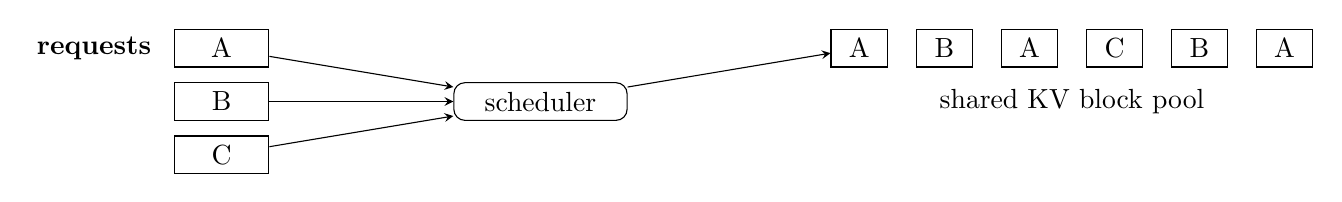
\begin{tikzpicture}[x=1.35cm,y=0.75cm,>=stealth]
\node at (-1.2,2.4) {\textbf{requests}};
\node[draw,minimum width=1.2cm] (a) at (0,2.4) {A};
\node[draw,minimum width=1.2cm] (b) at (0,1.5) {B};
\node[draw,minimum width=1.2cm] (c) at (0,0.6) {C};

\node[draw,rounded corners,minimum width=2.2cm] (sched) at (3.0,1.5) {scheduler};

\node[draw,minimum width=0.72cm] (k1) at (6.0,2.4) {A};
\node[draw,minimum width=0.72cm] (k2) at (6.8,2.4) {B};
\node[draw,minimum width=0.72cm] (k3) at (7.6,2.4) {A};
\node[draw,minimum width=0.72cm] (k4) at (8.4,2.4) {C};
\node[draw,minimum width=0.72cm] (k5) at (9.2,2.4) {B};
\node[draw,minimum width=0.72cm] (k6) at (10.0,2.4) {A};

\node at (8.0,1.5) {shared KV block pool};

\draw[->] (a) -- (sched);
\draw[->] (b) -- (sched);
\draw[->] (c) -- (sched);
\draw[->] (sched) -- (k1);
\end{tikzpicture}
\caption{Paged KV management allocates blocks from a shared pool rather than requiring one large contiguous reservation for each request.}
\label{fig:paged-kv}
\end{figure}

\subsubsection*{SGLang}

SGLang also targets efficient LLM serving but places additional emphasis on structured generation/runtime execution and reuse across repeated prompt prefixes.
The useful distinction is workload bias: applications with repeated prompt structure, branching model calls or agent-like execution can expose reuse and scheduling opportunities beyond one independent request.

Do not memorise one implementation feature as a permanent differentiator.
Serving systems copy successful ideas quickly.
Compare them by the stable design axes: scheduler, memory manager, supported models, kernel stack, parallelism, hardware support and operational ergonomics.

\subsubsection*{TensorRT-LLM}

TensorRT-LLM is NVIDIA's specialised LLM inference stack.
It combines optimised kernels, quantisation, KV-cache management, batching and multi-GPU execution with close coupling to NVIDIA hardware/software.

The advantage is access to aggressive hardware-specific optimisation.
The cost is a narrower hardware/runtime boundary and more deployment-specific optimisation work than a generic PyTorch path.

\begin{table}[ht]
\centering
\small
\begin{tabularx}{\textwidth}{>{\bfseries}p{2.3cm} X X X}
\toprule
Engine & Structural bias & Attractive when & Main trade-off \\
\midrule
vLLM & dynamic LLM requests should share GPU memory/compute efficiently & broad model serving with strong throughput and familiar API patterns & specialised inference runtime to operate and tune \\
SGLang & structured/repeated generation programs expose reuse and scheduling opportunities & complex LLM applications and serving workloads with repeated structure & runtime/programming model adds another abstraction \\
TensorRT-LLM & exploit NVIDIA-specific inference capabilities aggressively & NVIDIA deployment where maximum hardware-specific optimisation matters & tighter hardware coupling and build/tuning complexity \\
\bottomrule
\end{tabularx}
\caption{Inference engines solve the same underlying scheduling and memory problems with different system boundaries.}
\label{tab:llm-engines}
\end{table}

\begin{calloutmemoryhook}
An LLM inference engine is mostly a scheduler plus a KV-memory manager plus fast kernels.
\end{calloutmemoryhook}


\subsection{Inference engine versus inference server}

An \textbf{engine} decides how model computation executes efficiently.
A \textbf{server} decides how clients access one or more engines over a network.

A server adds concerns such as
\[
\text{routing}
+
\text{request queues}
+
\text{authentication}
+
\text{replicas}
+
\text{health checks}
+
\text{version rollout}
+
\text{observability}.
\]

NVIDIA Triton \textbf{Inference Server} belongs here and should not be confused with the Triton GPU-kernel language.
The names are similar; the abstraction levels are not.

\begin{table}[ht]
\centering
\small
\begin{tabularx}{\textwidth}{>{\bfseries}p{3.0cm} X X}
\toprule
System & Main job & Typical object it manages \\
\midrule
Triton language & write/compile GPU kernels & one custom operation/kernel \\
vLLM / SGLang / TensorRT-LLM & execute autoregressive models efficiently & model requests + KV state \\
Triton Inference Server & host model backends behind network APIs & models, versions, request queues \\
Ray Serve & compose and scale Python model/application deployments & replicas, deployments and request graph \\
KServe-like layer & Kubernetes-native serving lifecycle & declarative serving resources and rollout \\
\bottomrule
\end{tabularx}
\caption{Kernel compiler, inference engine and model server are different system layers.}
\end{table}


\subsection{Experiment lifecycle: MLflow}

Training code produces more than weights.
A result depends on code, data, preprocessing, configuration, random state and environment, as discussed in Section~2.16.

MLflow makes that experiment identity persistent:
\[
\underbrace{\text{parameters + metrics + artifacts + code/context}}_{\text{run}}
\rightarrow
\underbrace{\text{logged model}}_{\text{artifact}}
\rightarrow
\underbrace{\text{registered model version}}_{\text{lineage + controlled identity}}
\rightarrow
\underbrace{\text{deployment alias / rollout}}_{\text{operational choice}}.
\]

\textbf{Tracking} answers ``what happened in this run?''
The \textbf{Model Registry} answers ``which version of the model are we referring to, where did it come from, and which version should an environment use?''

\begin{figure}[ht]
\centering
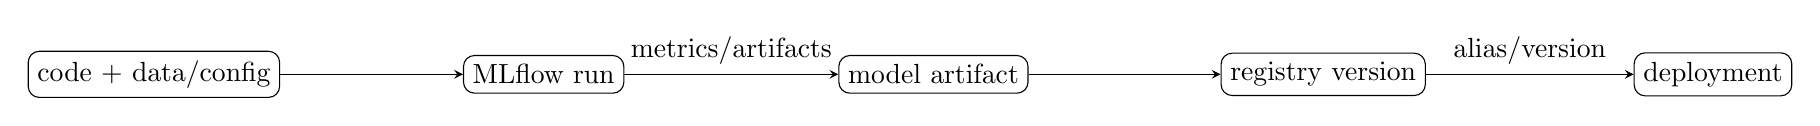
\begin{tikzpicture}[x=1.65cm,y=0.8cm,>=stealth]
\node[draw,rounded corners] (code) at (0,2) {code + data/config};
\node[draw,rounded corners] (run) at (3,2) {MLflow run};
\node[draw,rounded corners] (artifact) at (6,2) {model artifact};
\node[draw,rounded corners] (registry) at (9,2) {registry version};
\node[draw,rounded corners] (deploy) at (12,2) {deployment};

\draw[->] (code) -- (run);
\draw[->] (run) -- node[above]{metrics/artifacts} (artifact);
\draw[->] (artifact) -- (registry);
\draw[->] (registry) -- node[above]{alias/version} (deploy);
\end{tikzpicture}
\caption{Lifecycle tooling links a deployed artifact back to the experiment that produced it.}
\label{fig:mlflow-lineage}
\end{figure}

The trade-off is bookkeeping and infrastructure.
For a one-off notebook, a directory and a CSV may be sufficient.
Once multiple people, retraining jobs or production deployments depend on model identity, informal file naming becomes fragile.

\begin{calloutpracticaltip}
Log the information required to reproduce a decision, not every scalar merely because the API permits it.
\end{calloutpracticaltip}


\subsection{Managed model APIs: Bedrock and the ownership boundary}

A managed foundation-model service such as Bedrock moves the abstraction boundary upward.
Instead of operating a model server, the application calls a managed inference API.

\begin{figure}[ht]
\centering
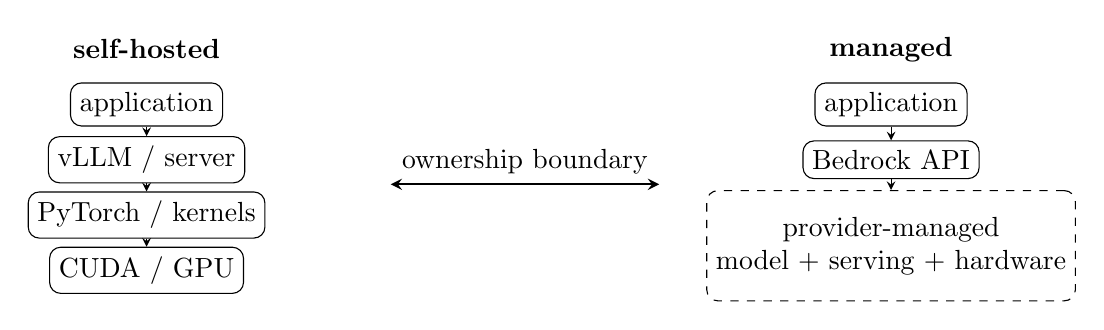
\begin{tikzpicture}[x=1.55cm,y=0.78cm,>=stealth]
\node at (0,4.4) {\textbf{self-hosted}};
\node[draw,rounded corners] (a1) at (0,3.5) {application};
\node[draw,rounded corners] (a2) at (0,2.6) {vLLM / server};
\node[draw,rounded corners] (a3) at (0,1.7) {PyTorch / kernels};
\node[draw,rounded corners] (a4) at (0,0.8) {CUDA / GPU};
\draw[->] (a1)--(a2);
\draw[->] (a2)--(a3);
\draw[->] (a3)--(a4);

\node at (6.1,4.4) {\textbf{managed}};
\node[draw,rounded corners] (b1) at (6.1,3.5) {application};
\node[draw,rounded corners] (b2) at (6.1,2.6) {Bedrock API};
\node[draw,dashed,rounded corners,minimum width=3.5cm,minimum height=1.4cm,align=center] (b3) at (6.1,1.2)
{provider-managed\\model + serving + hardware};
\draw[->] (b1)--(b2);
\draw[->] (b2)--(b3);

\draw[<->,thick] (2.0,2.2) -- node[above]{ownership boundary} (4.2,2.2);
\end{tikzpicture}
\caption{Managed APIs remove direct control of the lower serving stack in exchange for removing responsibility for operating it.}
\label{fig:managed-boundary}
\end{figure}

The central trade is
\[
\boxed{
\text{less infrastructure control}
\leftrightarrow
\text{less infrastructure responsibility}
}.
\]

The managed path reduces work around capacity planning, GPU provisioning, serving software, scaling and many failure modes.
In exchange, model availability, custom kernels, low-level scheduler behaviour, hardware placement and some cost/performance optimisations are controlled by the provider.

Bedrock and SageMaker also solve different default problems.
A Bedrock-like service primarily provides managed access to foundation-model capabilities.
A SageMaker-like platform is broader ML infrastructure for training, jobs, endpoints and models the user controls more directly.

\begin{calloutinductivebias}
If model execution is not the research variable, a managed model API can remove irrelevant systems work; if inference behaviour itself is the experiment, the same abstraction may hide the variable of interest.
\end{calloutinductivebias}


\subsection{LLM application orchestration: LangGraph}

A single model call needs little orchestration.
Complex applications introduce persistent state and control flow:

\[
\text{input}
\rightarrow
\text{model}
\rightarrow
\begin{cases}
\text{answer}\\
\text{call tool}\\
\text{ask another model}\\
\text{wait for approval}\\
\text{retry}\\
\text{branch}
\end{cases}
\rightarrow
\text{updated state}.
\]

At that point the application is naturally a graph/state-machine problem.
LangGraph-like systems make nodes, state transitions, persistence and resume/retry behaviour explicit.

\begin{figure}[ht]
\centering
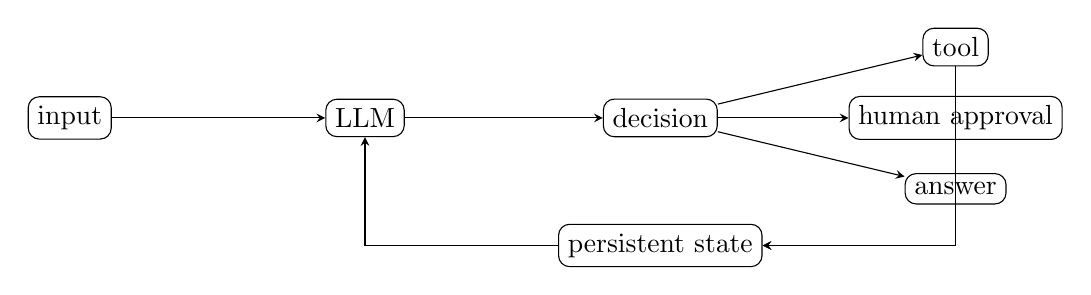
\begin{tikzpicture}[x=1.5cm,y=0.9cm,>=stealth]
\node[draw,rounded corners] (input) at (0,2) {input};
\node[draw,rounded corners] (llm) at (2.5,2) {LLM};
\node[draw,rounded corners] (route) at (5.0,2) {decision};
\node[draw,rounded corners] (tool) at (7.5,3) {tool};
\node[draw,rounded corners] (human) at (7.5,2) {human approval};
\node[draw,rounded corners] (answer) at (7.5,1) {answer};
\node[draw,rounded corners] (state) at (5.0,0.2) {persistent state};

\draw[->] (input)--(llm);
\draw[->] (llm)--(route);
\draw[->] (route)--(tool);
\draw[->] (route)--(human);
\draw[->] (route)--(answer);
\draw[->] (tool) |- (state);
\draw[->] (human) |- (state);
\draw[->] (state) -| (llm);
\end{tikzpicture}
\caption{Agent orchestration becomes useful when model calls are embedded inside explicit stateful control flow.}
\label{fig:langgraph}
\end{figure}

The alternative is ordinary Python.
That is often preferable when the workflow is small: fewer dependencies, easier debugging and no graph abstraction to learn.
A workflow framework earns its cost when persistence, branching, retries, resumability or inspection of long-running state become recurring requirements.

\begin{calloutmemoryhook}
Use an agent framework for stateful workflow complexity, not merely because an application calls an LLM.
\end{calloutmemoryhook}


\subsection{Complete deployment pipelines}

Individual APIs become easier to understand when followed through a complete data path.

\subsubsection*{Research experiment}

\[
\text{Parquet / dataset}
\rightarrow
\text{DataLoader}
\rightarrow
\text{PyTorch}
\rightarrow
\text{CUDA GPU}
\rightarrow
\text{MLflow run}
\rightarrow
\text{checkpoint + metrics}.
\]

The bottleneck can occur at every arrow.
Slow storage starves the accelerator; framework overhead creates too many small launches; an inefficient kernel wastes device time; lifecycle failures make the result irreproducible.

\subsubsection*{Distributed training}

\[
\text{object storage}
\rightarrow
\text{workers}
\rightarrow
\underbrace{\text{PyTorch + FSDP/DeepSpeed}}_{\text{training-state policy}}
\rightarrow
\underbrace{\text{NCCL}}_{\text{GPU communication}}
\rightarrow
\text{GPU cluster}
\rightarrow
\text{MLflow registry}.
\]

Ray may sit above the workers when the cluster must also schedule trials, preprocessing, data tasks or heterogeneous jobs.

\subsubsection*{Self-hosted LLM product}

\[
\text{user}
\rightarrow
\text{API/router}
\rightarrow
\text{application / LangGraph}
\rightarrow
\text{vLLM/SGLang/TensorRT-LLM}
\rightarrow
\text{CUDA}
\rightarrow
\text{GPU}
\rightarrow
\text{response}.
\]

End-to-end latency is still the decomposition from Section~2.14.2:
network, lookup, queueing, model compute and post-processing all remain visible.
A faster kernel does not repair a long queue.

\subsubsection*{Managed LLM product}

\[
\text{user}
\rightarrow
\text{application / LangGraph}
\rightarrow
\text{Bedrock-like API}
\rightarrow
\text{provider-managed model}
\rightarrow
\text{response}.
\]

This removes most model-serving components from the user's architecture but not application-level concerns such as prompt construction, caching, retries, evaluation, observability and product feedback.


\subsection{What competes and what composes}

A useful diagnostic is to ask whether two products control the \textbf{same decision}.
If not, they may compose.

\begin{table}[ht]
\centering
\small
\begin{tabularx}{\textwidth}{>{\bfseries}p{3.1cm} X X}
\toprule
Pair & Relationship & Reason \\
\midrule
PyTorch vs JAX & mostly alternatives & both express differentiable accelerator computation \\
Triton vs CUDA C++ & alternative abstraction levels & both can implement custom GPU kernels \\
DDP vs FSDP & alternatives for model-state distribution & replicate versus shard \\
FSDP + NCCL & compose & FSDP needs communication; NCCL performs collectives \\
Ray + FSDP & compose & Ray places workers; FSDP shards model state inside the training job \\
vLLM vs TensorRT-LLM & mostly alternatives & both can be the LLM inference runtime \\
vLLM + Triton language & compose internally/indirectly & inference engines may rely on specialised kernels \\
MLflow + PyTorch & compose & one trains; one records lifecycle state \\
LangGraph + Bedrock & compose & one orchestrates application state; one supplies managed model inference \\
Bedrock vs self-hosted vLLM & architectural alternatives & managed provider owns the lower stack versus user ownership \\
\bottomrule
\end{tabularx}
\caption{Competition is usually meaningful only between tools controlling the same system decision.}
\label{tab:compose-compete}
\end{table}


\subsection{API design as inductive bias}

The same inductive-bias framing used for models applies to software systems.

\begin{table}[ht]
\centering
\small
\begin{tabularx}{\textwidth}{>{\bfseries}p{2.8cm} X X}
\toprule
System & Assumption / bias & Consequence \\
\midrule
SciPy & problem matches a known numerical algorithm & mature solver is cheaper than implementing the method yourself \\
PyTorch & model can be expressed as tensor operations with autodiff & flexible gradient-based research loop \\
JAX & important computation can be expressed as transformable functions & compilation/vectorisation become composable program transformations \\
Triton & custom GPU work can be described efficiently at block/tile level & more control than framework ops with less boilerplate than CUDA C++ \\
NCCL & accelerator workers need collective tensor communication & topology-aware collectives become a reusable layer \\
Ray & work can be represented as schedulable tasks/actors with resource requirements & heterogeneous cluster execution becomes explicit \\
vLLM & many dynamic autoregressive requests share accelerator memory & scheduler and KV-memory management dominate serving design \\
MLflow & experiment identity must persist and be queried later & runs/artifacts/models become versioned operational objects \\
Bedrock & user prefers managed inference to owning the serving runtime & infrastructure disappears behind an API boundary \\
LangGraph & LLM application behaviour is stateful graph execution & branching, persistence and resume behaviour become explicit \\
\bottomrule
\end{tabularx}
\caption{Software abstractions encode assumptions about which operations should be easy.}
\label{tab:api-bias}
\end{table}


\subsection{How the stack evolved}

The history is an upward movement in abstraction with repeated downward escape hatches for performance.

\begin{table}[ht]
\centering
\small
\begin{tabularx}{\textwidth}{>{\bfseries}p{2.5cm} X X X}
\toprule
Step & What changed & Pressure & Remaining escape hatch \\
\midrule
Numerical libraries & reusable linear algebra/optimisation routines & stop reimplementing standard maths & lower-level C/Fortran kernels \\
Tensor frameworks & autodiff + accelerator tensors & express learned models directly & custom operators \\
Framework compilers & graph capture and fusion & recover performance lost to eager dispatch & custom Triton/CUDA kernels \\
Distributed runtimes & replication/sharding/collectives & one accelerator no longer sufficient & communication/runtime tuning \\
Inference engines & request scheduler + KV-memory system & autoregressive serving wastes memory/compute without specialised runtime & custom kernels / hardware-specific stacks \\
Managed model APIs & hide serving infrastructure & application teams do not always need infrastructure ownership & self-host when control/cost requires it \\
Agent/workflow runtimes & make state/control flow explicit & one model call became a long-running application workflow & ordinary Python for simpler paths \\
\bottomrule
\end{tabularx}
\caption{New abstractions remove repeated engineering work but retain lower-level routes when control becomes the research variable.}
\end{table}


\subsection{Degrees of experiment}

The software stack contains research variables just as the model does.

\begin{calloutdegreeexperiment}
\textbf{Framework:} eager versus compiled execution, static/dynamic shapes, dtype, fusion and checkpointing.
\newline
\textbf{Kernel:} tile/block size, memory layout, precision, fusion and implementation backend.
\newline
\textbf{Distributed training:} data/tensor/pipeline/sharded parallelism, worker placement, bucket size, offload and communication overlap.
\newline
\textbf{Inference:} KV-cache representation, batch/scheduling policy, prefill/decode separation, quantisation, speculative decoding, tensor/pipeline parallelism and replica count.
\newline
\textbf{Serving:} queue policy, batching window, autoscaling, routing, fallbacks and rollout policy.
\newline
\textbf{Lifecycle:} what is logged, model-version policy, reproducibility boundary and evaluation gate.
\newline
\textbf{Application:} managed versus self-hosted model, workflow graph, retry policy, tool routing and cache strategy.
\end{calloutdegreeexperiment}


\subsection{Researcher diagnostic}

When encountering an unfamiliar ML API, ask these questions in order:

\begin{enumerate}
\item \textbf{What enters and leaves?} Tensor, model, request, task, run, artifact or workflow state?
\item \textbf{Which operation becomes cheap?} Autodiff, compilation, communication, scheduling, serving, tracking or orchestration?
\item \textbf{What layer is hidden?} Python, kernel, network, cluster, server or cloud infrastructure?
\item \textbf{What control is lost?} Memory layout, kernel schedule, placement, model choice, retry semantics or lifecycle policy?
\item \textbf{What is the dominant bottleneck?} CPU/Python, memory bandwidth, GPU compute, GPU communication, queueing or network latency?
\item \textbf{Does another tool compete or compose?} Do they control the same decision?
\item \textbf{What fails?} Graph break, out-of-memory, collective hang, worker death, stale model version, timeout or workflow state loss?
\item \textbf{What can be varied experimentally?} Identify the configuration variables before accepting defaults.
\end{enumerate}

\begin{figure}[ht]
\centering
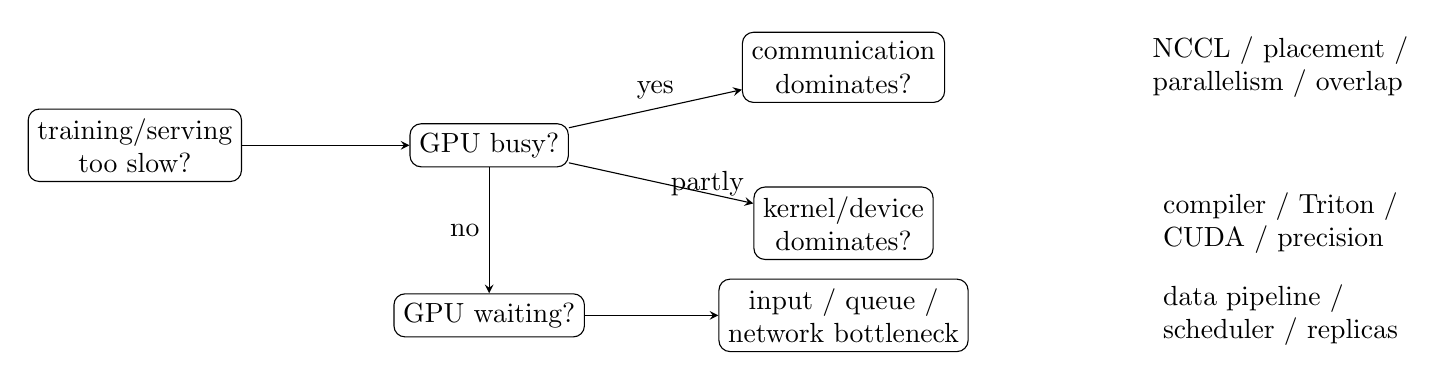
\begin{tikzpicture}[x=1.5cm,y=0.9cm,>=stealth]
\node[draw,rounded corners,align=center] (slow) at (0,3.5) {training/serving\\too slow?};
\node[draw,rounded corners,align=center] (gpu) at (3.0,3.5) {GPU busy?};
\node[draw,rounded corners,align=center] (comm) at (6.0,4.6) {communication\\dominates?};
\node[draw,rounded corners,align=center] (kernel) at (6.0,2.4) {kernel/device\\dominates?};
\node[draw,rounded corners,align=center] (input) at (3.0,1.1) {GPU waiting?};
\node[draw,rounded corners,align=center] (queue) at (6.0,1.1) {input / queue /\\network bottleneck};

\draw[->] (slow)--(gpu);
\draw[->] (gpu)-- node[above]{yes} (comm);
\draw[->] (gpu)-- node[right]{partly} (kernel);
\draw[->] (gpu)-- node[left]{no} (input);
\draw[->] (input)--(queue);

\node[align=left] at (9.7,4.6) {NCCL / placement /\\parallelism / overlap};
\node[align=left] at (9.7,2.4) {compiler / Triton /\\CUDA / precision};
\node[align=left] at (9.7,1.1) {data pipeline /\\scheduler / replicas};
\end{tikzpicture}
\caption{The relevant API depends on where the bottleneck lives; do not optimise a lower layer merely because it is technically interesting.}
\label{fig:api-diagnostic}
\end{figure}


\subsection{Knowledge boundary for an ML researcher}

The required depth is enough to identify the active layer, reason about bottlenecks and modify the variables relevant to an experiment.
Implementation depth below that boundary depends on role.

\begin{table}[ht]
\centering
\small
\begin{tabularx}{\textwidth}{>{\bfseries}p{3.3cm} X}
\toprule
Topic & Useful depth \\
\midrule
NumPy / SciPy & comfortable; recognise when a classical numerical routine is the correct tool \\
PyTorch & strong; tensors, autograd, modules, optimisers, device movement and profiling \\
JAX & comfortable; understand \texttt{grad}/\texttt{vmap}/\texttt{jit} and functional-state implications \\
\texttt{torch.compile} / XLA & conceptual-to-comfortable; graph capture, compilation cost, fusion and graph breaks \\
CUDA hardware model & strong intuition; memory hierarchy, kernels, thread/block execution and synchronisation \\
Triton kernels & recognise and modify simple kernels; deeper authoring for systems/performance roles \\
NCCL collectives & strong intuition; know AllReduce/AllGather/ReduceScatter and communication bottlenecks \\
DDP/FSDP/DeepSpeed & comfortable; choose replication/sharding strategy and diagnose memory/communication trade-offs \\
Ray & conceptual-to-comfortable; tasks, actors, resource scheduling and where it sits above ML frameworks \\
vLLM/SGLang/TensorRT-LLM & strong serving intuition; KV memory, batching, scheduling, quantisation and parallelism \\
MLflow & comfortable; runs, artifacts, lineage, model versions and rollback identity \\
Bedrock-like managed APIs & architectural; ownership/cost/control boundary matters more than memorising endpoint syntax \\
LangGraph-like orchestration & architectural; use when workflow state/control complexity justifies it \\
Kubernetes internals / cloud administration & recognise unless role-specific \\
Hand-written CUDA optimisation & specialist depth unless performance systems is the role \\
\bottomrule
\end{tabularx}
\caption{A researcher's knowledge boundary is systems reasoning first, product-specific administration second.}
\label{tab:api-knowledge-boundary}
\end{table}


\subsection{Final mental model}

The complete path for a self-hosted ML system can be read from top to bottom:

\[
\boxed{
\begin{array}{c}
\text{product / experiment}\\
\downarrow\\
\text{workflow and request API}\\
\downarrow\\
\text{model framework or inference engine}\\
\downarrow\\
\text{compiler and kernels}\\
\downarrow\\
\text{device runtime + communication}\\
\downarrow\\
\text{hardware}
\end{array}
}
\]

MLflow records what happened across the path.
Ray can schedule work across machines around the path.
A managed service such as Bedrock replaces a large lower portion of the path with a provider-owned boundary.

\begin{calloutintuition}
Do not learn ML APIs as brand names.
Locate the layer, identify the operation it makes cheap, then ask what control and failure modes the abstraction introduces.
\end{calloutintuition}